\section{Structure through equivalence}
%%%%%%%%%%%%%%%%%%%%%%%%%%%%%%%%%%%%%%%%%%%%%%%%%%%%%%%%%
\subsection{Motivation}

\draftnote{blue}{Include}{
Something about how extracting the global algebra provides potential for generalisation compared to learning each individual labelled transformation.
}

\newthought{Consider a world-agent} pair $\mathscr{W}$-$\mathscr{A}$.
Our algebra of actions $(\hat{A}^{*}, \circ)$ is a free monoid, which is the same for any world.
This free monoid $\hat{A}^{*}$ is the most general, and therefore the most structure free, monoid constructed from the atomic actions in $\hat{A}$ - its structure only depends on the atomic actions in $\hat{A}$\footnote{
In fact, any monoid generated by $\hat{A}$ can be obtained by imposing additional structure, in the form of relations, on $\hat{A}^{*}$, and so every monoid can be viewed as a quotient of $\hat{A}^{*}$ under some relation.
}.
However, we expect that there must be more structure we can tease out of our $(\hat{A}^{*}, \circ)$ since it appears that different worlds have different transformation structures.

Now remember the transformation structure of the world due to the actions of an agent is captured by the monoid action $(\hat{A}^{*}, \circ, \ast)$.
It would be useful if we could abstract how actions behave in the world from the individual world states by extracting aspects of the transformation structure of the world $\mathscr{W}$ into the monoid $(\hat{A}^{*}, \circ)$ through a relation.
Additionally, if we want to find other recognisable algebraic structures (e.g., groups, semigroups etc...) in the structure of worlds, we need a way of saying collections of transformations (i.e., the actions that are elements of $\hat{A}^{*}$) are the same in some way, otherwise, there is no way to satisfy the requirements of these algebras\footnote{
For example, for the group inverse property to be satisfied we need, for each $a \in \hat{A}^{*}$, an element $a'$ in $\hat{A}^{*}$ such that
\begin{align}
    & a' \circ a = e \\
    & a \circ a' = e.
\end{align}
where $e$ is the identity element.
}.

\newthought{So we want} a relation on the actions in $\hat{A}^{*}$ that (1) gives us a concept of sameness between actions (so we can satisfy requirements of algebraic structures that we want to find), and (2) captures some of the structure of the world in the monoid $(\hat{A}^{*}, \circ)$.
To do this we define an equivalence relation $\sim$ on the elements of $\hat{A}^{*}$; this equivalence relation enforces aspects of the structure of the world onto the free monoid $(\hat{A}^{*}, \circ)$ to give us a new algebra $(\hat{A}^{*}/\sim, \circ_{\sim})$ , where it is now possible to satisfy properties like the inverse condition.
We believe agents can gain a better understanding of the structure of the world though learning the structure of the algebras we will construct using equivalence relations.
In fact, we believe that when an agent is learning the transformation structure of a world, the agent is predominantly learning equivalence relations on $\hat{A}^{*}$ that reflect the transformation structure of the world.


%%%%%%%%%%%%%%%%%%%%%%%%%%%%%%%%%%%%%%%%%%%%%%%%%%%%%%%%%
\subsection{An equivalence relation $\sim$}

\newthought{We define an} equivalence relation on the elements of $\hat{A}^{*}$ that says two actions are equivalent (our sense of the actions being the same) if the actions lead to the same end world state when performed in any initial world state\footnote{
Our use of equivalence relations was inspired by \cite{caselles2020sensory}'s use of an equivalence relation to equate action sequences that produced the same end observation from an initial state \draftnote{blue}{(we discuss issues with \cite{caselles2020sensory}'s approach in section ???)}{}.
We realised that a global version of a similar equivalence relation is exactly the mathematical interpretation of the equality found in \cite{Higgins2018}.
}.
Formally, we define the equivalence $\sim$ as, for two actions $a, a' \in \hat{A}^{*}$,
\begin{equation}
    a \sim a' \iff a \ast w = a' \ast w \quad \text{ for all $w \in W$}.
\end{equation}


\begin{propositionE}
    $\sim$ is an equivalence relation on $\hat{A}^{*}$.
\end{propositionE}
\begin{proofE}
\begin{enumerate}
    \item \textbf{Reflexivity.}
    For any $a \in \hat{A}^{*}$, $a \ast w = a \ast w$ for all $w \in W$ (by reflexivity of equality). Hence $a \sim a$.
    
    \item \textbf{Symmetry.}
    Suppose $a \sim a'$ for $a, a' \in \hat{A}^{*}$.
    \begin{align}
        & a \sim a' \\
        \implies & a \ast w = a' \ast w \quad \text{for all $w \in W$} \\
        \implies & a' \ast w = a \ast w \quad \text{for all $w \in W$} \\
        \implies & a' \sim a
    \end{align}
    
    \item \textbf{Transitivity.}
    Suppose $a \sim a'$ and $a' \sim a''$ for $a, a', a'' \in \hat{A}^{*}$.
    \begin{equation}
        a \sim a' \implies a \ast w = a' \ast w \quad \text{for all $w \in W$}
    \end{equation}
    and
    \begin{equation}
        a' \sim a'' \implies a' \ast w = a'' \ast w \quad \text{for all $w \in W$}.
    \end{equation}
    Therefore,
    \begin{align}
        & a \ast w = a' \ast w \text{ and } a' \ast w = a'' \ast w \quad \text{for all $w \in W$} \\
        \implies & a \ast w = a'' \ast w \quad \text{for all $w \in W$} \\
        \implies & a \sim a''
    \end{align}

    \item \textbf{Conclusion.}
    Since $\sim$ is reflexive, symmetric, and transitive, $\sim$ is an equivalence relation on $\hat{A}^{*}$.
\end{enumerate}
\end{proofE}

\begin{notation}
    We denote the the equivalence class of an action $a \in \hat{A}^{*}$ due to the equivalence relation $\sim$ by  $[a]_{\sim}$.
\end{notation}

We define the canonical projection map $\pi_{\sim}: \hat{A}^{*} \to \hat{A}^{*}/\sim$ that sends actions in $\hat{A}^{*}$ to their equivalence classes $[a]_{\sim}$ under $\sim$ in the quotient set $\hat{A}^{*}/\sim$:
\begin{equation}
\begin{aligned}
    & \pi_{\sim}: \hat{A}^{*} \to \hat{A}^{*}/\sim \quad \text{such that} \\
    & \pi_{\sim}(a) = [a]_{\sim} \quad \text{for all $a \in \hat{A}^{*}$}
\end{aligned}
\end{equation}
where the equivalent classes $[a]_{\sim}$ are the sets
\begin{equation}
	[a]_{\sim} = \{ a' \in \hat{A}^{*} \mid a' \sim a \}
\end{equation}
and the quotient set $\hat{A}^{*}/\sim$ is the collection of all such equivalence classes
\begin{equation}
    \hat{A}^{*}/\sim = \{ [a]_{\sim} \mid a \in \hat{A}^{*} \}.
\end{equation}

We can view the projection map $\pi_{\sim}$ as collapsing actions in $\hat{A}/\sim$ that are indistinguishable in terms of their effect on $W$ into a single representative element in the quotient set $\hat{A}^{*}/\sim$\footnote{
    When we define an equivalence $\sim$ on $\hat{A}^{*}$ to get the set $\hat{A}^{*}/\sim$, we can think of our set $\hat{A}^{*}$ `folding over' on itself to make elements of $\hat{A}^{*}$ that are equivalent stick together.
}.
Since $\sim$ is an equivalence relation, the collection $\hat{A}^{*}/\sim$ of equivalence classes forms a partition of $\hat{A}^{*}$; this means that\footnote{
Formally, $\hat{A}^{*}/\sim$ has the properties of
\begin{enumerate}
    \item \textbf{Coverage.}
    Every action $a \in \hat{A}^{*}$ belongs to some equivalence class $[a]_{\sim}$;

    \item \textbf{Disjointness.}
    For any two actions $a, a' \in \hat{A}^{*}$, either $[a]_{\sim} = [b]_{\sim}$ or $[a]_{\sim} \cap [b]_{\sim} = \emptyset$.
\end{enumerate}
}
\begin{enumerate}
    \item every action in $\hat{A}^{*}$ belongs to an equivalence class in $\hat{A}^{*}/\sim$;
    \item every action in $\hat{A}^{*}$ belongs to exactly one equivalence class in $\hat{A}^{*}/\sim$.
\end{enumerate}

%%%%%%%%%%%%%%%%%%%%%%%%%%%%%%%%%%%%%%%%%%%%%%%%%%%%%%%
\paragraph{Composition of equivalent actions.}
\newthought{We define the} composition operator $\circ_{\sim}$ on the elements in $\hat{A}^{*}/\sim$ using our action composition operator $\circ$ as
\begin{equation}
	\begin{aligned}
		 & \circ_{\sim}: (\hat{A}^{*}/\sim) \times (\hat{A}^{*}/\sim) \to (\hat{A}^{*}/\sim) \quad \text{such that} \\
		 & [a']_{\sim} \circ_{\sim} [a]_{\sim} = [a' \circ a]_{\sim} \quad \text{for $a,a' \in \hat{A}^{*}$}.
	\end{aligned}
\end{equation}

We need to show that the operation $\circ_{\sim}$ on the equivariance classes does not depend on the representative element chosen for those classes; this means we can consistently use any element of an equivalence class as a representative of that class (i.e., the operation $\circ_{\sim}$ is well-defined).

\begin{propositionE}
    \label{prp:circ_sim_well_defined}
    $\circ_{\sim}$ is well-defined on $\hat{A}^{*}/\sim$.
\end{propositionE}
\begin{proofE}
\begin{enumerate}
    \item \textbf{Problem.}
    For $\circ_{\sim}$ to be well-defined on $\hat{A}^{*}/\sim$, we need\footnote{
        \textbf{Well-definedness requirement.}
        An operation on a quotient set
        \begin{equation}
            (\hat{A}^{*}/\sim) \times (\hat{A}^{*}/\sim) \to \hat{A}^{*}/\sim
        \end{equation}
        is \emph{well-defined} if take different representatives of the same equivalence classes doesn't change the resulting equivalence class.
        Mathematically,
        \begin{equation}
        \begin{aligned}
            & [a]_{\sim} = [b]_{\sim} \; \text{and} \; [a']_{\sim} = [b']_{\sim} \\
            \implies & [a' \circ a]_{\sim} = [b' \circ b]_{\sim}
        \end{aligned}
        \end{equation}
    }
    \begin{equation}
    \begin{aligned}
        & [a]_{\sim} = [b]_{\sim} \text{ and } [a']_{\sim} = [b']_{\sim} \\
        \implies & [a' \circ a]_{\sim} = [b' \circ b]_{\sim}
    \end{aligned}
    \end{equation}

    \item \textbf{Initial assumptions.}
    For $a, b \in \hat{A}^{*}$:
    \begin{align}
        & a \sim b \\
        \implies & a \ast w = b \ast w \quad \text{for all } w \in W
    \end{align}
    and, for $a', b' \in \hat{A}^{*}$,
    \begin{align}
        & a' \sim b' \\
        \implies & a' \ast w = b' \ast w \quad \text{for all } w \in W
    \end{align}

    \item \textbf{Goal.}
    We want to show $[a' \circ a]_{\sim} = [b' \circ b]_{\sim}$.
    \begin{align}
                    & [a' \circ a]_{\sim} = [b' \circ b]_{\sim}                               \\
      \Rightarrow{} & (a' \circ a) \sim (b' \circ b)                                          \\
      \Rightarrow{} & (a' \circ a) \ast w = (b' \circ b) \ast w \quad \text{for all } w \in W
    \end{align}

    \item \textbf{Proof.}
    We have:
    \begin{equation}
      (a' \circ a) \ast w = a' \ast (a \ast w).
    \end{equation}
    Similarly, we have:
    \begin{equation}
      (b' \circ b) \ast w = b' \ast (b \ast w).
    \end{equation}
    Since $a \sim b$, we have $a \ast w = b \ast w$ for all $w \in W$.
    Therefore,
    \begin{align}
        (a' \circ a) \ast w & = a' \ast (a \ast w)\\
        & = a' \ast (b \ast w)
    \end{align}
    Since $a' \sim b'$, we have $a' \ast w = b' \ast w$ for all $w \in W$.
    Therefore,
    \begin{align}
        (a' \circ a) \ast w & = b' \ast (b \ast w) \\
        & = (b' \circ b) \ast w.
    \end{align}

    \item \textbf{Conclusion.}
    We have shown that $(a' \circ a) \ast w = (b' \circ b) \ast w$, and therefore $(a' \circ a) \sim (b' \circ b)$, and hence $\circ_{\sim}$ is well-defined on $\hat{A}^{*}/\sim$.
\end{enumerate}
\end{proofE}


Since the composition operator $\circ_{\sim}$ induced by the equivalence relation $\sim$ is well-defined, $\sim$ is a \emph{congruence relation}\footnote{
    A congruence relation is an equivalence relation on an algebraic structure that preserves the structure's operations.
    
    In the case of $\circ$, $\circ_{\sim}$ can be thought of as the composition operator $\circ$ after it has been pulled through the map $\pi_{\sim}$ unaffected.
} on the monoid $(\hat{A}^{*}, \circ)$.

\begin{propositionE}
    \label{prp:circ_sim_closed}
    $\circ_{\sim}: (\hat{A}^{*}/\sim) \times (\hat{A}^{*}/\sim) \to \hat{A}^{*}/\sim$ is closed.
\end{propositionE}
\begin{proofE}
    Let $[a]_{\sim}, [b]_{\sim}$ be arbitrary elements in $\hat{A}^{*}/\sim$.
    Choose arbitrary representatives of $[a]_{\sim}$ and $[b]_{\sim}$ and denote them $a, b \in \hat{A}^{*}$.
    By definition of $\circ$, $a \circ b \in \hat{A}^{*}$, and so $[a \circ b]_{\sim} \in \hat{A}^{*}/\sim$.
    By definition of $\circ_{\sim}$, $[a]_{\sim} \circ_{\sim} [b]_{\sim} = [a \circ b]_{\sim}$, and so $\circ_{\sim}$ is closed.
\end{proofE}

%%%%%%%%%%%%%%%%%%%%%%%%%%%%%%%%%%%%%%%%%%%%%%%%%%
\paragraph{Effect of equivalent actions on world states.}
\newthought{We define the} induced action effect operator $\ast_{\sim}$ on $\hat{A}^{*}/\sim$ as
\begin{equation}
\begin{aligned}
    & \ast_{\sim}: (\hat{A}^{*}/\sim) \times W \to W \quad \text{such that} \\
    & [a]_{\sim} \ast_{\sim} w = a \ast w
\end{aligned}
\end{equation}

\begin{propositionE}
    $\ast_{\sim}$ is well-defined on $\hat{A}^{*}/\sim$.
\end{propositionE}
\begin{proofE}
\begin{enumerate}
    \item \textbf{Goal.}
    To prove that $\ast_{\sim}$ is well-defined, we need to show that if two actions $a, b \in \hat{A}^{*}$ are equivalent (i.e., $a \sim b$), then they have the same effect on any world state $w$.
    We want to prove that
    \begin{equation}
        a \sim b \implies [a]_{\sim} \ast_{\sim} w = [b]_{\sim} \ast_{\sim} w
    \end{equation}
    Which is equivalent to proving that:
    \begin{equation}
        a \ast w = b \ast w.
    \end{equation}

    \item \textbf{Proof.}
    Suppose $a \sim b$.
    By definition of $\sim$ we have
    \begin{align}
        & a \sim b \\
        \implies & a \ast w = b \ast w \quad \text{for all } w \in W
    \end{align}

    By definition of $\ast_{\sim}$, the effect of $[a]_{\sim}$ on a world $w$ is given by
    \begin{equation}
      [a]_{\sim} \ast_{\sim} w = a \ast w
    \end{equation}
    Similarly, the effect of $[b]_{\sim}$ on a world $w$ is given by
    \begin{equation}
      [b]_{\sim} \ast_{\sim} w = b \ast w
    \end{equation}

    Combining the above, we have
    \begin{align}
        & a \sim b \\
        \implies & a \ast w = b \ast w \quad \text{for all } w \in W \\
        \implies & [a]_{\sim} \ast_{\sim} w = [b]_{\sim} \ast_{\sim} w \quad \text{for all } w \in W
    \end{align}

    Therefore, the definition of $\ast_{\sim}$ does not depend on the representative chosen, and so $\ast_{\sim}$ is well-defined on $\hat{A}^{*}/\sim$.
\end{enumerate}
\end{proofE}

Since $\ast_{\sim}$ and $\circ_{\sim}$ are both well-defined, the equivalence relation $\sim$ is a congruence relation on the monoid action $(\hat{A}^{*}, \circ, \ast)$. 

\begin{notation}
    Now we have proved that $\ast_{\sim}$ is well-defined on $\hat{A}^{*}/\sim$ we can denote $\ast_{\sim}$ by $\ast$ where it is obvious what we mean\footnote{
    $\ast_{\sim}$ can be thought of as the composition operator $\ast$ after it has been pulled through the map $\pi_{\sim}$ unaffected.
    }.
\end{notation}


%%%%%%%%%%%%%%%%%%%%%%%%%%%%%%%%%%%%%%%%%%%%%%%
\subsection{New structures from $\sim$}

\newthought{Applying our projection} map $\pi_{\sim}$ to the structures $(\hat{A}^{*}, \circ)$, $(\hat{A}^{*}, \circ, \ast)$, and $\mathcal{T}_{\hat{A}^{*}}$ gives us these new structures:\footnote{
    Technically $\pi_{\sim}(\text{ }\mathcal{T}_{\hat{A}^{*}}\text{ }) = \mathcal{T}_{\hat{A}^{*}/\sim}$ implies that the functions $f_{a}$ induced by individual actions $a \in \hat{A}^{*}$ correspond exactly to the functions $f_{[a]_{\sim}}$ induced by the equivalence classes in $\hat{A}^{*}/\sim$.
    We will prove this soon.
}
\begin{align}
	 & \pi_{\sim}(\text{ }(\hat{A}^{*}, \circ)\text{ }) = (\hat{A}^{*}/\sim, \circ_{\sim})                    \\
	 & \pi_{\sim}(\text{ }(\hat{A}^{*}, \circ, \ast)\text{ }) = (\hat{A}^{*}/\sim, \circ_{\sim}, \ast_{\sim}) \\
	 & \pi_{\sim}(\text{ }\mathcal{T}_{\hat{A}^{*}}\text{ }) = \mathcal{T}_{\hat{A}^{*}/\sim}
\end{align}


\newthought{Applying the equivalence relation} $\sim$ to the free monoid $(\hat{A}^{*}, \circ)$ gives the quotient monoid $(\hat{A}^{*}/\sim, \circ_{\sim})$\footnote{
	$(\hat{A}^{*}/\sim, \circ_{\sim})$ is the homomorphic image of $(\hat{A}^{*}, \circ)$ through the projection $\pi_{\sim}$.
}, whose elements are the equivalence classes $[a]_{\sim}$ for all $a \in \hat{A}^{*}$.

\begin{propositionE}
\label{prp:circ_sim_associative}
    $\circ_{\sim}$ is associative on $\hat{A}^{*}/\sim$.
\end{propositionE}
\begin{proofE}
Associativity of $\circ_{\sim}$ comes from the associativity of $\circ$.
\begin{align}
         & ([a'']_{\sim} \circ_{\sim} [a']_{\sim}) \circ_{\sim} [a]_{\sim} \\
    = \; & [a'' \circ a']_{\sim} \circ_{\sim} [a]_{\sim}                   \\
    = \; & [ (a'' \circ a') \circ a ]_{\sim}                               \\
    = \; & [ a'' \circ (a' \circ a) ]_{\sim}                               \\
    = \; & [a'']_{\sim} \circ_{\sim} [a' \circ a]_{\sim}                   \\
    = \; & [a'']_{\sim} \circ_{\sim} ([a']_{\sim} \circ_{\sim} [a]_{\sim})
\end{align}
\end{proofE}


\begin{propositionE}
\label{prp:A_sim_identity}
    $[\varepsilon]_{\sim}$ is the identity element of $(\hat{A}^{*}/\sim, \; \circ_{\sim})$, where $\varepsilon$ is the empty action.
\end{propositionE}
\begin{proofE}
    From the definition of $\varepsilon$,
    \begin{align}
        & \varepsilon \circ a = a \quad \text{for all $a \in \hat{A}^{*}$} \\
        & a \circ \varepsilon = a \quad \text{for all $a \in \hat{A}^{*}$}
    \end{align}
    Therefore, for any $a \in \hat{A}^{*}$, we have
    \begin{align}
        [\varepsilon]_{\sim} \circ_{\sim} [a]_{\sim} & = [\varepsilon \circ a]_{\sim} \\
        & = [a]_{\sim}
    \end{align}
    Similarly, for any $a \in \hat{A}^{*}$, we have
    \begin{align}
        [a]_{\sim} \circ_{\sim} [\varepsilon]_{\sim} & = [a \circ \varepsilon]_{\sim} \\
        & = [a]_{\sim}
    \end{align}
    Therefore, $[\varepsilon]_{\sim}$ is the identity element of $(\hat{A}^{*}/\sim, \; \circ_{\sim})$.
\end{proofE}


\begin{propositionE}
\label{prp:A_sim_is_monoid}
    $(\hat{A}^{*}/\sim, \circ_{\sim})$ is a monoid.
\end{propositionE}
\begin{proofE}
\begin{enumerate}
    \item \textbf{Closure and well-definedness.}
    $\circ_{\sim}$ is well-defined on $\hat{A}^{*}/\sim$ from \cref{prp:circ_sim_well_defined} and closed from \cref{prp:circ_sim_closed}.

    \item \textbf{Associativity.}
    Given by \cref{prp:circ_sim_associative}.

    \item \textbf{Identity Element.}
    Given by \cref{prp:A_sim_identity}.

    \item \textbf{Conclusion.}
    The structure $(\hat{A}^{*}/\sim, \circ_{\sim})$ is a monoid.
\end{enumerate}
\end{proofE}


Now we will show that $\pi_{\sim}$ preserves the monoid structure of $(\hat{A}^{*}, \circ)$, and so $\pi_{\sim}$ is a monoid homomorphism.

\begin{propositionE}
    $\pi_{\sim}$ is a monoid homomorphism from $(\hat{A}^{*}, \circ)$ to $(\hat{A}^{*}/\sim, \circ_{\sim})$.
\end{propositionE}
\begin{proofE}
\begin{enumerate}
    \item \textbf{Preservation of the Operation.}
    For any $a, a' \in \hat{A}^{*}$, the projection $\pi_{\sim}$ satisfies:
    \begin{align}
      \pi_{\sim}(a \circ a') & = [a \circ a']_{\sim}                 \\
                          & = [a]_{\sim} \circ_{\sim} [a']_{\sim} \\
                          & = \pi_{\sim}(a) \circ_{\sim} \pi_{\sim}(a')
    \end{align}
    Thus:
    \begin{equation}
      \pi_{\sim}(a \circ a') = \pi_{\sim}(a) \circ_{\sim} \pi_{\sim}(a').
    \end{equation}

    \item \textbf{Preservation of the Identity Element.}
    The identity element in $(\hat{A}^{*}, \circ)$ is $\varepsilon$, and the identity element in $(\hat{A}^{*}/\sim, \circ_{\sim})$ is $[\varepsilon]_{\sim}$.
    The projection satisfies:
    \begin{equation}
      \pi_{\sim}(\varepsilon) = [\varepsilon]_{\sim}.
    \end{equation}

    \item \textbf{Conclusion.}
    The projection $\pi_{\sim}$ is a monoid homomorphism.
\end{enumerate}
\end{proofE}


If the number of distinct effects on $W$ is finite, then $(\hat{A}^{*}/\sim, \circ_{\sim})$ will have a finite number of elements.


\newthought{Our monoid action} $(\hat{A}^{*}, \circ, \ast)$ also survives the application of the equivalence relation $\sim$ to become a quotient monoid action $(\hat{A}^{*}/\sim, \circ_{\sim}, \ast_{\sim})$.

\begin{propositionE}
    $(\hat{A}^{*}/\sim, \circ_{\sim}, \ast_{\sim})$ is a monoid action of $(\hat{A}^{*}/\sim, \circ_{\sim})$ on the set $W$.
\end{propositionE}
\begin{proofE}
\begin{enumerate}
    \item \textbf{Compatibility.}
    The action effect operator $\ast_{\sim}$ is compatible with the composition operator $\circ_{\sim}$ since:
    \begin{equation}
        ([a']_{\sim} \circ_{\sim} [a]_{\sim}) \ast_{\sim} w = [a']_{\sim} \ast_{\sim} ([a]_{\sim} \ast_{\sim} w) \quad \text{for all } [a]_{\sim}, [a']_{\sim} \in \hat{A}^{*}/\sim, \, w \in W.
    \end{equation}
    
    \textit{Proof:} By the definitions of $\circ_{\sim}$ and $\ast_{\sim}$, we have:
    \begin{align}
        ([a']_{\sim} \circ_{\sim} [a]_{\sim}) \ast_{\sim} w & = [a' \circ a]_{\sim} \ast_{\sim} w                   \\
        & = (a' \circ a) \ast w                                 \\
        & = a' \ast (a \ast w)                                  \\
        & = [a']_{\sim} \ast_{\sim} ([a]_{\sim} \ast_{\sim} w).
    \end{align}
    Therefore, the compatibility condition holds.
    
    \item \textbf{Identity action.}
    The identity element $[\varepsilon]_{\sim}$ acts as the identity on $W$:
    \begin{equation}
        [\varepsilon]_{\sim} \ast_{\sim} w = w \quad \text{for all } w \in W.
    \end{equation}
    
    \textit{Proof:} Using the definition of $\ast_{\sim}$ and knowing that $\varepsilon$ is the empty action sequence, we get:
    \begin{align}
        [\varepsilon]_{\sim} \ast_{\sim} w & = \varepsilon \ast w \\
        & = w.
    \end{align}
    Thus, $[\varepsilon]_{\sim}$ acts as the identity on $W$.
    
    \item \textbf{Conclusion.}
    We have verified both the compatibility and the identity conditions, and so $(\hat{A}^{*}/\sim, \circ_{\sim}, \ast_{\sim})$ is a monoid action on the set $W$.
\end{enumerate}
\end{proofE}


\newthought{Now we will} explore the effect that applying the equivalence relation $\sim$ has to our transformation monoid $\mathcal{T}_{\hat{A}^{*}}$.
We begin by considering how $\sim$ affects the functions $f_{a}$ that make up $\mathcal{T}_{\hat{A}^{*}}$.

\begin{propositionE}
\label{prp:equivalence_relation_gives_equal_action_functions}
    $a \sim a' \iff f_{a}(w) = f_{a'}(w)$ for all $w \in W$.
\end{propositionE}
\begin{proofE}
\begin{enumerate}
    \item \textbf{Forward direction.}
    Let $a \sim a'$. By the definition of $\sim$, this means:
    \begin{equation}
        a \ast w = a' \ast w \quad \text{for all } w \in W.
    \end{equation}
    The functions $f_{a}$ and $f_{a'}$ are defined as:
    \begin{equation}
        f_{a}(w) = a \ast w, \quad f_{a'}(w) = a' \ast w.
    \end{equation}
    From the assumption $a \ast w = a' \ast w$, we have:
    \begin{equation}
        f_{a}(w) = f_{a'}(w) \quad \text{for all } w \in W.
    \end{equation}
    Therefore, the functions $f_{a}$ and $f_{a'}$ are identical:
    \begin{equation}
        f_{a} = f_{a'}.
    \end{equation}

    \item \textbf{Reverse direction.}
    The functions $f_{a}$ and $f_{a'}$ are defined as:
    \begin{equation}
        f_{a}(w) = a \ast w, \quad f_{a'}(w) = a' \ast w.
    \end{equation}
    Since $f_{a}(w) = f_{a'}(w)$, it follows that:
    \begin{equation}
        a \ast w = a' \ast w \quad \text{for all } w \in W.
    \end{equation}
    By the definition of $\sim$, we conclude that:
    \begin{equation}
        a \sim a'
    \end{equation}

    \item \textbf{Conclusion.}
    Combining both directions, we have:
    \begin{equation}
        a \sim a' \iff f_{a}(w) = f_{a'}(w) \quad \text{for all } w \in W.
    \end{equation}
\end{enumerate}
\end{proofE}

A consequence of \cref{prp:equivalence_relation_gives_equal_action_functions} is that the equivalence relation $\sim$ is the \emph{kernel} $\operatorname{ker}(\phi)$\footnote{
The kernel $\operatorname{ker}(\phi)$ of a monoid homomorphism $M$ is defined as
\begin{equation}
    \operatorname{ker}(\phi) = \{(a,b) \in M \times M \mid \phi(a) = \phi(b) \}.
\end{equation}
} of $\phi: \hat{A}^{*} \to \mathcal{T}_{\hat{A}^{*}}$:
\begin{equation}
    \operatorname{ker}(\phi) = \sim
\end{equation}
since
\begin{equation}
    a \sim a' \iff f_{a} = f_{a'} \iff \phi(a) = \phi(a').
\end{equation}
We now have another way to show that the equivalence relation $\sim$ is a congruence on $(\hat{A}^{*}, \circ)$ because, since kernels of homomorphisms are congruences, it follows that $\sim$ is a congruence on $(\hat{A}^{*}, \circ)$; it also follows that any operation induced on the quotient $\hat{A}^{*}/\operatorname{ker}(\phi) = \hat{A}^{*}/\sim$ is well-defined (e.g., $\circ$).

As we did with $\ast$, we can curry the action $\ast_{\sim}: (\hat{A}^{*}/\sim) \times W \to W$
\begin{equation}
    \operatorname{Curry}: (\ast_{\sim}: (\hat{A}^{*}/\sim) \times W \to W) \to (f_{[a]_{\sim}}: W \to W)
\end{equation}
to obtain a collection of functions
\begin{equation}
\begin{aligned}
     & \mathcal{T}_{\hat{A}^{*}/\sim} = \{ f_{[a]_{\sim}} \mid a \in \hat{A}^{*} \} \quad \text{such that} \\
     & f_{[a]_{\sim}}(w) = [a]_{\sim} \ast w = a \ast w \quad \text{for $a \in \hat{A}^{*}$}.
\end{aligned}
\end{equation}
The set $\mathcal{T}_{\hat{A}^{*}/\sim}$ is the set $\mathcal{T}_{\hat{A}^{*}}$ but with identical functions in $\mathcal{T}_{\hat{A}^{*}}$ now collapsed into a single representative in $\mathcal{T}_{\hat{A}^{*}/\sim}$.

\begin{propositionE}
\label{prp:transformations_are_submonoid_of_full_transformation_monoid_on_W}
    $\mathcal{T}_{\hat{A}^{*}/\sim}$ is a monoid.
\end{propositionE}
\begin{proofE}
    $\mathcal{T}_{\hat{A}^{*}}$ is a monoid from \cref{prp:T_is_monoid}.
    From \cref{prp:equivalence_relation_gives_equal_action_functions}, the equivalence relation $\sim$ identifies actions that yield the same function; therefore, the induced set $\mathcal{T}_{\hat{A}^{*}/\sim}$ consists of unique functions from $W$ to $W$.
    The operation of function composition is well-defined on these equivalence classes, and so inherits associativity and the identity element $f_{\varepsilon}$ from $\mathcal{T}_{\hat{A}^{*}}$.
    Therefore, $\mathcal{T}_{\hat{A}^{*}/\sim}$ is a monoid.
\end{proofE}

Similar to what we did with $\phi: \hat{A}^{*} \to \mathcal{T}_{\hat{A}^{*}}$, we define a map
\begin{equation}
	\begin{aligned}
		 & \Phi : \hat{A}^{*}/\sim \to \text{End}(W) \quad \text{where} \\
		 & \Phi([a]_{\sim}) = f_{[a]_{\sim}}
	\end{aligned}
\end{equation}
\footnote{$\text{End}(W)$ is the set of functions from $W$ to itself.
	Functions from a set to itself are called \emph{endomorphisms}.}

\begin{propositionE}
    $\Phi$ is an injective homomorphism.
\end{propositionE}
\begin{proofE}
\begin{enumerate}
    \item \textbf{$\Phi$ is a homomorphism.}
    \begin{enumerate}
        \item \textbf{Goal.}
        We want, for all $[a]_{\sim}, [a']_{\sim} \in \hat{A}^{*}/\sim$,
        \begin{equation}
            \Phi([a']_{\sim} \circ_\sim [a]_{\sim}) = \Phi([a']_{\sim}) \cdot \Phi([a]_{\sim})
        \end{equation}
        
        \item \textbf{Proof.}
        From the definition of $\Phi$ we have
        \begin{align}
            \Phi([a']_{\sim} \circ_\sim [a]_{\sim}) & = \Phi([a' \circ a]_{\sim}) \\
            & = f_{[a' \circ a]_{\sim}}.
        \end{align}
        Now, for any $w \in W$,
        \begin{align}
            f_{[a' \circ a]_{\sim}}(w) & = (a' \circ a) \ast w \\
            & = a' \ast (a \ast w)  \\
            & = f_{[a']_{\sim}}(f_{[a]_{\sim}}(w)) \\
            & = (f_{[a']_{\sim}} \cdot f_{[a]_{\sim}})(w).
        \end{align}
        Therefore,
        \begin{align}
            \Phi([a']_{\sim} \circ_\sim [a]_{\sim}) & = f_{[a' \circ a]_{\sim}} \\
            & = f_{[a']_{\sim}} \cdot f_{[a]_{\sim}} \\
            & = \Phi([a']_{\sim}) \cdot \Phi([a]_{\sim})
        \end{align}
        Therefore, $\Phi$ preserves the monoid operation and so is a monoid homomorphism.
    \end{enumerate}
    
    \item \textbf{$\Phi$ is injective.}
    \begin{enumerate}
        \item \textbf{Goal.}
        We want to show that:
        \begin{equation}
            \Phi([a]_{\sim}) = \Phi([a']_{\sim}) \implies [a]_{\sim} = [a']_{\sim}
        \end{equation}
        
        \item \textbf{Proof.}
        Suppose $\Phi([a]_{\sim}) = \Phi([a']_{\sim})$ for some $a, a' \in \hat{A}^{*}$.
        \begin{align}
            & \Phi([a]_{\sim}) = \Phi([a']_{\sim}) \\
            \implies & f_{[a]_{\sim}} = f_{[a']_{\sim}} \\
            \implies & f_{[a]_{\sim}}(w) = f_{[a']_{\sim}}(w) \quad \text{for all $w \in W$}
        \end{align}
        From \cref{prp:equivalence_relation_gives_equal_action_functions},
        \begin{align}
            & f_{[a]_{\sim}}(w) = f_{[a']_{\sim}}(w) \quad \text{for all $w \in W$} \\
            \implies & a \ast w = a' \ast w \quad \text{for all $w \in W$} \\
            \implies & a \sim a' \\
            \implies & [a]_{\sim} = [a']_{\sim}
        \end{align}
        Therefore, $\Phi$ is injective.
    \end{enumerate}
\end{enumerate}
\end{proofE}


\newthought{We will now} use the injectivity of $\Phi$ to establish an upper bound on the number of elements in $\hat{A}^{*}/\sim$.

\begin{propositionE}
    $|\hat{A}^{*}/\sim| \leq |W|^{|W|}$.
\end{propositionE}
\begin{proofE}
\begin{enumerate}
    \item \textbf{Relation between $\hat{A}^{*}/\sim$ and endofunctions on $W$.}
    Since $\Phi$ is injective, there is a one-to-one correspondence between elements of $\hat{A}^{*}/\sim$ and their images in $\text{End}(W)$ under $\Phi$.
    Each $[a]_{\sim} \in \hat{A}^{*}$ corresponds uniquely to the function $f_{[a]_{\sim}} \in \text{End}(W)$.

    \item \textbf{Counting the number of functions in $\text{End}(W)$.}
    Every function from $W$ to $W$ is an endomorphism, so each element $w \in W$ can be mapped to any of the $|W|$ elements in $W$.
    Since there are $|W|$ elements in $W$, the total number of functions from $W$ to $W$ is
    \begin{equation}
        |\text{End}(W)| = |W|^{|W|}.
    \end{equation}

    \item \textbf{Establishing the upper bound.}
    Since $\Phi$ is injective, the number $|\hat{A}^{*}/\sim|$ of elements in $\hat{A}^{*}/\sim$ is less than or equal to the number of functions from $W$ to $W$, and so
    \begin{equation}
        |\hat{A}^{*}/\sim| \leq |\text{End}(W)| = |W|^{|W|}
    \end{equation}
\end{enumerate}
\end{proofE}

If we restrict the image of the map $\Phi$ to only the functions from $W$ to $W$ that are due to an action in $\hat{A}^{*}$, then the restricted map will become a bijection (and therefore an isomorphism).
The image required for this restriction is exactly the restriction to our set $\mathcal{T}_{\hat{A}^{*}/\sim}$ (i.e., $\Phi(\hat{A}^{*}/\sim) = \mathcal{T}_{\hat{A}^{*}/\sim}$).

\begin{propositionE}
\label{prp:A_to_T_isomorphism}
    The restriction of $\Phi$ to the image $\mathcal{T}_{\hat{A}^{*}/\sim}$
    \begin{equation}
    \begin{aligned}
        & \Phi_{R} : \hat{A}^{*}/\sim \to \mathcal{T}_{\hat{A}^{*}/\sim} \quad \text{where} \\
        & \Phi_{R}([a]_{\sim}) = f_{[a]_{\sim}}
    \end{aligned}
    \end{equation}
    is an isomorphism\footnote{
    \Cref{prp:transformations_are_submonoid_of_full_transformation_monoid_on_W,prp:A_to_T_isomorphism} mean that the transformations generated by the actions in $\hat{A}^{*}$ form a sub-monoid of the full transformation monoid on $W$; the full transformation monoid on $W$ is $\text{End}(W)$.
    }.
\end{propositionE}
\begin{proofE}
    To prove that $\Phi_{R}$ is an isomorphism we need to show that $\Phi$ is injective, surjective and a homomorphism.
    \begin{enumerate}
    \item \textbf{Homomorphism.}
    This follows from the fact that $\Phi$ is a homomorphism.
    
    \item \textbf{Injective.}
    This follows from the fact that $\Phi$ is injective.
    
    \item \textbf{Surjective.}
    We have that
    \begin{equation}
        \Phi(\hat{A}^{*}/\sim) = \mathcal{T}_{\hat{A}^{*}/\sim}.
    \end{equation}
    Therefore, $\Phi_{R}$ maps $\hat{A}^{*}/\sim$ onto $\mathcal{T}_{\hat{A}^{*}/\sim}$; in other words, for every $f_{[a]_{\sim}} \in \mathcal{T}_{\hat{A}^{*}/\sim}$, there exists an $[a]_{\sim} \in \hat{A}^{*}/\sim$ such that $\Phi_{R}([a]_{\sim}) = f_{[a]_{\sim}}$.

    \item \textbf{Conclusion.}
    Since $\Phi_{R}$ is a homomorphisms that is both injective and surjective, it is an isomorphism.
\end{enumerate}
\end{proofE}

From \cref{prp:A_to_T_isomorphism}, we have that $(\hat{A}^{*}/\sim, \circ_{\sim})$ is isomorphic to $(\mathcal{T}_{\hat{A}^{*}/\sim}, \cdot)$\footnote{
    Since $\sim = \operatorname{ker}(\phi)$, this actually follows directly from the First Isomorphism Theorem for Monoids.
}
\begin{equation}
    (\hat{A}^{*}/\sim, \circ_{\sim}) \cong (\mathcal{T}_{\hat{A}^{*}/\sim}, \cdot),
\end{equation}
where $\cdot$ is the composition of functions.

This means that the structure enforced on the free monoid $(\hat{A}^{*}, \circ)$ and the transformation monoid $(\mathcal{T}_{\hat{A}^{*}}, \cdot)$ by applying the equivalence relation $\sim$ has caused these structures to collapse into the same structure.

%%%%%%%%%%%%%%%%%%%%%%%%%%%%%%%%%%%%%%%%%%%%%%%
\section{
Example: the equivalence condition on \texorpdfstring{$\mathscr{W}_{\alpha}$}{the toy world}
 }\label{sec:the_equivalence_condition_on_example_world}

\newthought{Now let's see} what happens with our example world $\mathscr{W}_{\alpha}$ when we apply the equivalence relation $\sim$. \Cref{fig:2x2_cyclical_equivalence_min_actions} shows what happens to \cref{fig:2x2_cyclical_labelling_with_min_actions} when we apply our equivalence relation $\sim$ to our example world-agent pair $\mathscr{W}_{\alpha}$-$\mathscr{A}$.
Note that for $\mathscr{W}_{\alpha}$-$\mathscr{A}$, we have $1 \sim \varepsilon$ and so the equivalence class $[1]_{\sim}$ of the no-op action $1 \in \hat{A}^{*}$ acts as the identity action of $(\hat{A}^{*}/\sim, \circ_{\sim})$.

\begin{figure}[H]
    \centering
    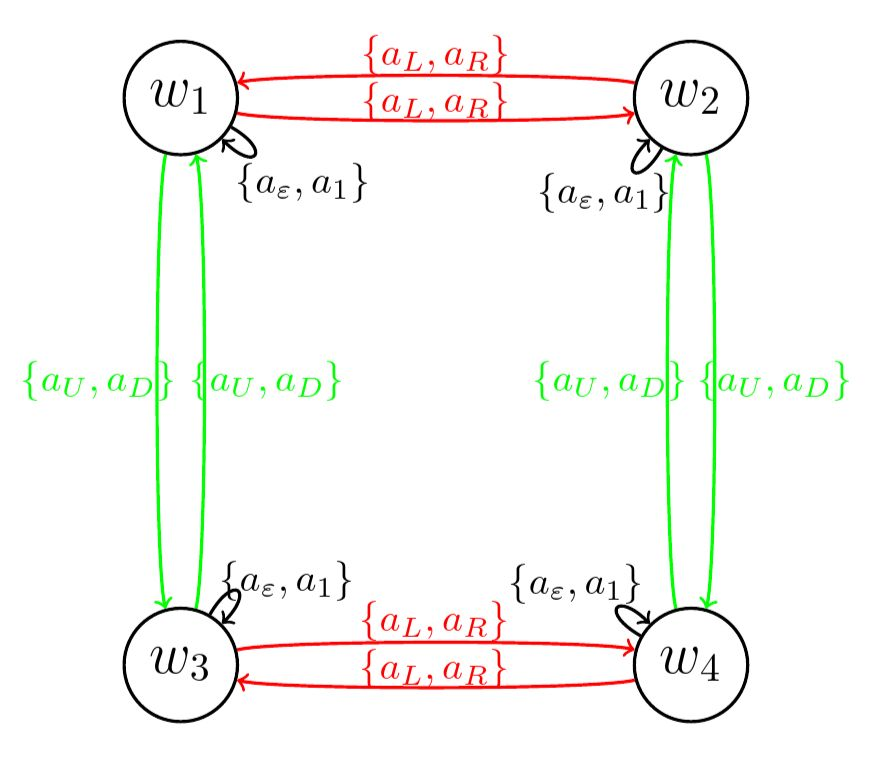
\includegraphics[width=0.75\linewidth]{2MathematicalFramework/Images/2x2_cyclical_equivalence_min_actions.jpeg}
    \caption{
    World diagram showing the equivalence classes under $\sim$ for the atomic actions and the empty action for the world-agent pair $\mathscr{W}_{\alpha}$-$\mathscr{A}$.
    \draftnote{purple}{PS}{
    Similar to \cref{fig:2x2_cyclical_labelling_with_min_actions}, put $\hat{A}^{*}$ diagram on the left with a $\pi_{\sim}$ labelled arrow pointing to the current figure on the right.
    }
    }
    \label{fig:2x2_cyclical_equivalence_min_actions}
\end{figure}

\draftnote{purple}{PS: Consider}{
\begin{enumerate}
    \item Diagram of map showing actions being sent to their equivalence classes under $\sim$: $D_{A}$ -($l$)-> $\hat{A}^{*}$ -($\pi_{A}$)-> $\hat{A}^{*}/\sim$.
\end{enumerate}
}

\whendraft{
\draftnote{red}{whendraft start}{}
%%%%%%%%%%%%%%%%%%%%%%%%%%%%%%%%%%%%%%%%
\section{
Equivalence on transformations
\draftnote{blue}{V0.5}{}
}

\draftnote{red}{Include}{
\begin{enumerate}
    \item (Put as footnote if there is no time) Equivalence relation $\sim$ for transformations and how it compares to equivalence relation $\sim$ for actions.
    \item Cannot apply the labelling map to $D/\sim$ to get $\hat{A}^{*}/\sim$.
    \item I think $\sim$ on $D$ matches the $\sim_{w}$'s.
\end{enumerate}
}

A natural analogue of our equivalence relation $\sim$ on actions is an equivalence relation, also denoted by $\sim$, on the transformations $D$ that equates two transforms is they both have the same sources and the same targets.
Formally, for $d, d' \in D$,
\begin{equation}
    d \sim d' \iff s(d) = s(d') \text{ and } t(d) = t(d')
\end{equation}
\draftnote{red}{whendraft end}{}
}

%%%%%%%%%%%%%%%%%%%%%%%%%%%%%%%%%%%%%%%%
\section{
Converting other equivalence relations
\texorpdfstring{to $\sim$}{}
\draftnote{blue}{V0.5}{}
}
\draftnote{red}{Include}{
\begin{enumerate}
    \item Formalism this section.
    \item Empirical example (using our algorithm).
    \item We can convert this into category theory quite easily I think (disjoint union).
\end{enumerate}
}

If we have another equivalence relation $\sim'$ on the actions in $\hat{A}^{*}$, we can transform the world $\mathscr{W}$ that $\sim'$ is being applied to and so harness what we have derived for the equivalence relation $\sim'$.

For example, let $\sim_{(t)}$ be defined as, for two actions $a, a' \in \hat{A}^{*}$,
\begin{align}
    & a \sim_{(t)} a' \iff a \ast w = a' \ast w \quad \text{ for all $w \in W$} \quad \text{and} \\
    & |a| \bmod t = |a'| \bmod t
\end{align}
We can transform any world $\mathscr{W}$, which we want to apply $\sim_{(t)}$ to, to a world $\mathscr{W}'$ when applying $\sim$ will produce the same algebraic structures as we would produce from applying $\sim_{(t=2)}$ to $\mathscr{W}$.
We do this by indexing each world state with the time\footnote{
Here we're taking time to be the number of atomic actions that have been performed from a given start time.
} $t \bmod 2$ that that world state can be visited at; then we split each world state with more than one index into that many new world states in $\mathscr{W}'$ connected with the relevant transformations with atomic action labels.
